%----------------------------------------------------------------------------------------
%	PACKAGES AND OTHER DOCUMENT CONFIGURATIONS
%----------------------------------------------------------------------------------------

\documentclass[twoside]{article}

\usepackage{graphicx} % Required for inserting images
\usepackage[english]{babel} % Dictionary

\usepackage{amsmath, amssymb, amsmath, amsthm} % Math 

\usepackage{enumitem} % lists
\usepackage{pifont} % for special lists

\usepackage{graphicx} % Graphics
\usepackage{float} % insert images fluently

\usepackage{changes} % to mark changes in the text
\usepackage{soul} % to mark changes in the text

\usepackage{csquotes} % cite a source
\usepackage{ifoddpage} % for \checkoddpage and \ifoddpage

%---------------------------------------------------------------------------------------
%	MARGIN SETTINGS
%----------------------------------------------------------------------------------------

% \geometry{
% 	paper=a4paper, % Change to letterpaper for US letter
% 	inner=2.5cm, % Inner margin
% 	outer=3.8cm, % Outer margin
% 	bindingoffset=.5cm, % Binding offset
% 	top=1.5cm, % Top margin
% 	bottom=1.5cm, % Bottom margin
% 	showframe, % Uncomment to show how the type block is set on the page
% }

\usepackage{setspace}
\usepackage{geometry} % margin settings
\geometry{a4paper, margin=2.5cm}

% Bibliography
\usepackage[
    backend = biber, 
    style = numeric, 
    sorting = nty 
]{biblatex}
\addbibresource{references.bib} %adds the source file
% backend = biber sorts the bibliography
% style = numberic uses numbers for the sources, can also be alphabetic, authoryear, authortitle etc. 
% sorting = nty sorts the sources by name, title, year, also possible nyt, nyvt (volume), none etc. for more information see overleaf documentation, Bibliography management in LaTeX
\bibliography{plain}
\bibliography{ref}

%----------------------------------------------------------------------------------------
% Theorems
%----------------------------------------------------------------------------------------
\theoremstyle{plain} % boldface title, italicized body
\newtheorem{theorem}{Theorem}[section]

\theoremstyle{definition} % boldface title, Roman body
\newtheorem{definition}[theorem]{Definition}

\newtheorem{corollary}[theorem]{Corollary}
\newtheorem{proposition}[theorem]{Proposition}
\newtheorem{property}[theorem]{Property}
\newtheorem{lemma}[theorem]{Lemma}
\newtheorem{example}[theorem]{Example}

\theoremstyle{remark} % italicized title, Roman body
\newtheorem*{remark}{Remark}

%----------------------------------------------------------------------------------------
% Shortcuts
%----------------------------------------------------------------------------------------

\newcommand*\N{\mathbb{N}}
\newcommand*\Z{\mathbb{Z}}
\newcommand*\Q{\mathbb{Q}}
\newcommand*\R{\mathbb{R}}

\newcommand*\x{\mathbf{x}}
\newcommand*\y{\mathbf{y}}

\newcommand{\cmmnt}[1]{}
%----------------------------------------------------------------------------------------
% Title Page
%----------------------------------------------------------------------------------------
\begin{document}

\begin{titlepage}
    \centering
    
\includegraphics[width=0.3\textwidth]{Figures/Uni_Zuerich_Siegel.svg.png}\par\vspace{1cm}
    {\scshape\LARGE University of Zurich \par}
    \vspace{1.5cm}
    {\huge\bfseries Master Thesis \par}
    \vspace{1cm}
    {\Large Title Thesis \par}
    \vspace{2cm}
    {\large Author: Keerthiga Rajakumar \par}
    \vspace{0.5cm}
    {\large Supervisor: Marius Furter \par}
    \vfill
    {\large \today\par}
    \date{\today}

\end{titlepage}


% Front  
\pagenumbering{roman}
\tableofcontents
\cleardoublepage


% Main 
\pagenumbering{arabic}
\setcounter{page}{1}

%----------------------------------------------------------------------------------------
%\singlespacing

\section{Basic Probability}
\begin{itemize}
    \item Conditional probability distribution % Kalman Filter
    \item Gaussian random walk
\end{itemize}

\subsection{Probabilistic state space models}
% Definition is from the book Bayesian filtering and smoothing` by Simo Särkkä page 51.
\begin{definition}[Probabilistic state space models]
A probabilistic state space model or non-linear filtering model consists of a sequence of conditional probability distributions: 
\begin{align}
&\mathbf{x}_t \sim p(\mathbf{x}_t \mid \mathbf{x}_{t-1}), \nonumber \\
&\mathbf{y}_t \sim p(\mathbf{y}_t \mid \mathbf{x}_t),
\end{align}
for $t=1,2,...$, where 
\begin{itemize}
    \item $\mathbf{x}_t \in \mathbb{R}^n$ is the state of the system at time step $t$,
    \item $\mathbf{y}_t \in \mathbb{R}^m$ is the measurement at time step $t$, 
    \item $p(\mathbf{x}_t\mid \mathbf{x}_{t-1})$ is the dynamic model which describes the stochastic dynamics of the system. The dynamic model can be a probability density, a counting measure or a combination of them depending on whether the state $\mathbf{x}_t$ is continuous, discrete, or hybrid. 
    \item $p(\mathbf{y}_t\mid \mathbf{x}_t)$ is the measurement model, which is the distribution of measurements given the state. 
\end{itemize}
The model is assumed to be Markovian, which means that it has the following two properties. 
\end{definition}

% Property is from the book Bayesian filtering and smoothing` by Simo Särkkä page 52.
\begin{property}[Markov property of states]
The states $\{\mathbf{x}_t: t = 0,1,2,...\}$ form a Markov sequence (or Markov chain if the state is discrete). This Markov property means that $\mathbf{x}_t$ (and actually the whole future $\mathbf{x}_{t+1}, \mathbf{x}_{t+2},...$) given $\mathbf{x}_{t-1}$ is independent of anything that has happened before the time step $t-1$: 

\begin{equation}\label{eq: Markov property of states}
   p(\mathbf{x}_t\mid \mathbf{x}_{1:t-1},\mathbf{y}_{1:t-1} )=  p(\mathbf{x}_t\mid \mathbf{x}_{t-1}).
\end{equation}

\noindent Also the past is independent of the future given the present: 

\begin{equation}
   p(\mathbf{x}_{t-1}\mid \mathbf{x}_{t:T},\mathbf{y}_{t:T} )=  p(\mathbf{x}_{t-1}\mid \mathbf{x}_t).
\end{equation}
\end{property}

% Property is from the book Bayesian filtering and smoothing` by Simo Särkkä page 52.
\begin{property}[Conditional independence of measurements]
The current measurement $\mathbf{y}_t$ given the current state $\mathbf{x}_t$ is conditionally independent of the measurement and state histories: 
\begin{equation}\label{eq: Conditional independence of measurements}
p(\mathbf{y}_t \mid \mathbf{x}_{1:t}, \mathbf{y}_{1:t-1}) = p(\mathbf{y}_t \mid \mathbf{x}_t).    
\end{equation}
\end{property}

%------------------------------------------------------------------------
%------------------------------------------------------------------------

\noindent Let us start with an example to get a better understanding of the definition.
\begin{example}[Tracking a drone's position and velocity in 2D]
Imagine you are watching a drone fly over an open field. You want to keep track of where the drone is and how fast it is moving in both directions, vertically and horizontally. At each point in time, the drone has a position and a velocity. To represent this, we define something called the \textbf{state} of the system. The state is a list of numbers that describe everything we need to know about the drone.

To model this, we organize these numbers into a state vector, which lists all the quantities we want to keep track of: 
\[ \mathbf{x}_t = \begin{bmatrix}
    x_t \\ y_t \\ v_{x,t} \\ v_{y,t}
\end{bmatrix},\]

where
\begin{itemize}
    \item $(x_t,y_t)$ represent the position of the drone at time step $t$,
    \item $(v_{x,t},v_{y,t})$ represent the velocity in the $x$ and $y$ directions. 
\end{itemize}

%------------------------------------------------------------------------

\medskip
Let's consider what we can actually observe. Suppose we have a GPS sensor that tells us the drone's position at each time step. This means we can measure the position, but not the velocity. In other words, we know where the drone is but not how fast it is moving. The \textbf{observation model} describes how the measurements we receive are connected to the drone's actual position \textcolor{orange}{(data we can observe)} and velocity \textcolor{orange}{(important but hidden variable from direct measurement).} 

The observation model is written like this: 

\begin{equation}\label{eq: observation model}
\textbf{y}_t = \textbf{H}\textbf{x}_{t}+\textbf{r}_{t},   
\end{equation}

where 
\begin{itemize}
    \item $\textbf{y}_t$ is the measurement at time step $t$,
    \item $\textbf{H}$ is a matrix that shows \textcolor{orange}{how the state vector relates to the observed measurements},
    \item $\mathbf{r}_t$ represents small random measurement noise and is modeled as Gaussian, i.e. $\mathbf{r}_t \sim \mathcal{N}(0, \mathbf{R})$. In our example, this corresponds to the GPS error. 
\end{itemize}

The observation matrix \textbf{H} is: 
\[\mathbf{H} = \begin{bmatrix}
   1 & 0 & 0 & 0\\
   0 & 1 & 0 & 0\\   
\end{bmatrix}\]

The matrix has non-zero entries in the first and second columns since we can only observe position. This means: 

\[\mathbf{y}_t = \begin{bmatrix}
   x_t \\
   y_t \\ 
\end{bmatrix} + \textbf{r}_t\]

%-----------------------------------------------------------------------------------------

\medskip 
Now we make a simple assumption about how the drone moves. % Has not to be a straight line - M1706: We assume it keeps flying at about the same speed in a straight line
\textcolor{orange}{We assume it flies with approximately constant velocity.} This means its future position depends on where it is now and how fast it is going. The position alone would not be enough because the drone might be hovering in place or racing across the field. If we know the current state, we can make a good guess about what the next state will be. 

This is called the state \textbf{transition model}. It tells us how the drone's state changes from moment to moment. We include some randomness since movement is not always perfect, e.g.~the wind might push the drone a little off course. 

The transition model is written like this: 
\begin{equation}\label{eq: transition model}
\textbf{x}_t = \textbf{A}\textbf{x}_{t-1}+\textbf{q}_{t-1},   
\end{equation}

where 
\begin{itemize}
    \item $\textbf{x}_t$ is the state at time step $t$,
    \item $\textbf{A}$ is a matrix that describes how position and velocity are updated, 
    \item $\mathbf{q}_{t-1}$ represents small random measurement noise and is modeled as Gaussian, i.e. $\mathbf{q}_{t-1} \sim \mathcal{N}(0, \mathbf{Q})$. In our example, this would be a wind pushing the drone off course. 
\end{itemize}

In our example, this noise can affect either the position or the velocity. It can also affect both but we'll concentrate on these two cases. In the following, we will take a closer look on both cases. 

\begin{itemize}
    \item{1. Case: Position noise only:} We assume uncertainty arises mainly from small movements in the drone's position, e.g.\~ minor GPS shifts, while the velocity remains constant. The noise vector then looks like:
    \[\mathbf{q}_{t-1} = \begin{bmatrix}
        q_x \\
        q_y \\
        0 \\
        0
    \end{bmatrix},\]
    where $q_x$ and $q_y$ are Gaussian with mean $0$ and variance $\sigma_\text{pos}^2$ and the covariance matrix: 
    \[\mathbf{Q}=\begin{bmatrix}
        \sigma_\text{pos}^2 & 0 & 0 & 0 \\
        0 & \sigma_\text{pos}^2 & 0 & 0 \\
        0 & 0 & 0 & 0 \\
        0 & 0 & 0 & 0 
    \end{bmatrix}\]
    Here the drone drifts around over the field but keeps the same speed. 
    
    \item{2. Case: Velocity noise only:} This time we assume the position evolves smoothly but the drone's velocity or direction may change slightly, e.g.\~due to a breeze. Then:
    \[\mathbf{q}_{t-1}= \begin{bmatrix}
        0 \\
        0 \\
        q_{v,x} \\
        q_{v,y}
    \end{bmatrix}\]
    Now the drone flies smoothly but its velocity changes rather over time. 
\end{itemize}
\end{example}

% Note to myself: write code and play with q and see what happens
%-----------------------------------------------------------------------------------------
%-----------------------------------------------------------------------------------------




%\cleardoublepage


\newpage
\section{Bayesian filtering equations and exact solutions}
\subsection{Introduction to Bayesian filtering}
Bayesian filtering provides a structured way to estimate the state of a system that changes over time and can only be observed through noisy data. The system’s state usually includes time-dependent variables that describe its condition at each moment. However, measurements are often inaccurate because of noise, which creates uncertainty. On top of that, the system’s behavior over time can be affected by random changes or errors in the model, known as process noise.
\\
Bayesian filtering uses all observations up to the current time to estimate the system’s current state. Bayesian smoothing goes a step further by also using future observations to get better estimates of past states. Both filtering and smoothing are key tools in time series analysis and are used in many different fields.


% More generally, Bayesian filtering uses a set of recursive equations that work for both simple (linear-Gaussian) and more complex (nonlinear or non-Gaussian) models. The filtering process has two main steps:
% \begin{itemize}
%     \item A prediction step, which estimates the state based on the previous state and the system’s dynamics.
%     \item An update step, which incorporates the new observation to refine the state estimate.
% \end{itemize}

\subsection{Bayesian filtering equations}
\begin{theorem}[Bayesian filtering equations]
The recursive equations (the Bayesian filter) for computing the predicted distribution $p(\mathbf{x}_t \mid \mathbf{y}_{1:t-1})$ and the filtering distribution $p(\mathbf{x}_t \mid \mathbf{y}_{1:t})$ at the time step $t$ are given by the following Bayesian filtering equations.
\begin{itemize}
    \item \textbf{Initialization} The recursion starts from the prior distribution $p(\mathbf{x}_0)$
    \item \textbf{Prediction step} The predictive distribution of the state $\mathbf{x}_t$ at the time $t$, given the dynamic model, can be computed by the Chapman-Kolmogorov equation
    \[p(\mathbf{x}_t \mid \mathbf{y}_{1:t-1}) = \int p(\mathbf{x}_t \mid \mathbf{x}_{t-1})p(\mathbf{x}_{t-1} \mid \mathbf{y}_{1:t-1})d\mathbf{x}_{t-1}.\]
    \item \textbf{Update step} Given the measurement $\mathbf{y}_t$ at time step $t$ the posterior distribution of the state $\mathbf{x}_t$ can be computed by Bayes' rule
    \[p(\mathbf{x}_t\mid \mathbf{y}_{1:t}) = \frac{1}{Z_t}\textbf{ }p(\mathbf{y}_t \mid \mathbf{x}_t)\textbf{ }p(\mathbf{x}_t\mid \mathbf{y}_{1:t-1}),\]
    where the normalization constant $Z_t$ is given as 
    \[Z_t = \int p(\mathbf{y}_t \mid \mathbf{x}_t) \textbf{ }p(\mathbf{x}_t\mid \mathbf{y}_{1:t-1}) \textbf{ }d\mathbf{x}_t\]
\end{itemize}
The integrals are replaced with summations if the components of the state are discrete. 
\end{theorem}

\begin{proof}
For the proof, check pages 55 and 56 in the book `Bayesian filtering and smoothing' by Simo Särkkä. 
\end{proof}

\begin{example}[Estimating the Drone's Position with Bayesian Filtering]
    
\end{example}


\subsection{Exact solutions in Bayesian filtering}


\subsection{Advantages and Disadvantages of Bayesian Filtering}

% Zahlenbeispiel machen 
%\cleardoublepage


\newpage
\section{Kalman filter}
\subsection{The Kalman filter}
A well-known Bayesian filter is the Kalman filter, which gives the closed form solution to the Bayesian filtering equations. It gives an efficient way to estimate the state of a linear system with Gaussian noise.

The Kalman filter model is given by:

\begin{align}\label{eq:Kalman filter}
    \mathbf{x}_k &= \mathbf{A}_{k-1}\mathbf{x}_{k-1}+\mathbf{q}_{k-1}, \nonumber\\
    \mathbf{y}_k &= \mathbf{H}_k\mathbf{x}_k+\mathbf{r}_k
\end{align}

where 
\begin{itemize}
    \item $\mathbf{x}_k$ is the hidden state at time $k$,
    \item $\mathbf{A}_{k-1}$ is the state transition matrix,
    \item $\mathbf{1}_{k-1}$ represent the process noise (assumed to be Gaussian),
    \item $\mathbf{y}_k$ is the measurement at time $k$,
    \item $\mathbf{H}_k$ is the observation matrix, and
    \item $\mathbf{r}_k$ is the measurement noise (also assumed to be Gaussian).
\end{itemize}

The filter operates in two steps:
\begin{itemize}
    \item \textbf{Prediction}: The current state is predicted using the system model.
    \item \textbf{Update (correction)}: This prediction is corrected using the new measurement.
\end{itemize}

This mix of predicting and updating helps the filter follow the system’s state over time, even when the measurements are noisy.

The Kalman filter is widely used in various fields, including:
\begin{itemize}
    \item \textbf{Navigation}: Tracking planes, ships, and spacecraft
    \item \textbf{Robotics}: Helping robots know their position
    \item \textbf{Finance}: Modeling stock prices
    \item \textbf{Weather}: Predicting weather patterns
    \item \textbf{Phones}: Improving GPS location
\end{itemize}

% These methods are used in fields such as navigation, aerospace, space engineering, telecommunications, remote sensing, audio signal processing, control systems, and financial modeling, where the accurate estimation of dynamic system variables, either in real time or retrospectively, is important. 
% \\

\begin{theorem}[Kalman filter]
The Bayesian filtering equations for the linear filtering model \eqref{eq:Kalman filter} can be evaluated in closed form and the resulting distributions are Gaussian:    

\begin{align}\label{eq:Kalman filter distributions}
    p(\mathbf{x}_k\mid\mathbf{y}_{1:k-1})&= N(\mathbf{x}_k\mid\mathbf{m}_k^-,\mathbf{P}_k^-),\nonumber \\
    p(\mathbf{x}_k\mid\mathbf{y}_k)&= N(\mathbf{x}_k\mid\mathbf{m}_k,\mathbf{P}_k),\nonumber \\
    p(\mathbf{y}_k\mid\mathbf{y}_{1:k-1})&= N(\mathbf{y}_k\mid\mathbf{H}_k\mathbf{m}_k^-,\mathbf{S}_k).
\end{align}
The parameters of the distributions above can be computed with the following Kalman filter prediction and update steps.

\begin{itemize}
    \item The prediction step is
    \begin{align}
        \mathbf{m}_k^- &= \mathbf{A}_{k-1}\mathbf{m}_{k-1}, \nonumber\\
        \mathbf{P}_k^- &= \mathbf{A}_{k-1}\mathbf{P}_{k-1}\mathbf{A}_{k-1}^\top + \mathbf{Q}_{k-1}
    \end{align}

    \item The update step is
    \begin{align}
        \mathbf{v}_k &= \mathbf{y}_k - \mathbf{H}_k\mathbf{m}_k^- \nonumber\\
        \mathbf{S}_k &= \mathbf{H}_k\mathbf{P}_k^-\mathbf{H}_{k}^\top + \mathbf{R}_k \nonumber\\
        \mathbf{K}_k &= \mathbf{P}_k^-\mathbf{H}_k^\top\mathbf{S}_k^{-1} \nonumber\\
        \mathbf{m}_k &= \mathbf{m}_k^- + \mathbf{K}_k\mathbf{v}_k \nonumber\\
        \mathbf{P}_k &= \mathbf{P}_k^- - \mathbf{K}_k\mathbf{S}_k \mathbf{K}_k^\top
    \end{align}
\end{itemize}

The recursion is started from the prior mean $\mathbf{m}_0$ and covariance $\mathbf{P}_0$.
\end{theorem}

\begin{proof}
For the proof, check pages 57 and 58 in the book `Bayesian filtering and smoothing' by Simo Särkkä. 
\end{proof}



% what is a Kalman Filter and its meaning, applications, why relevant in my thesis

% mathematical background, state space representation, Gaussian noise assumptions, recursive Bayesian estimation (predict-update cycle), introduce predition and update step, covariance matrices

% derivation of the Kalman Fitler Equations, present the KF algorithm step-by-step

% discussion of assumptions and limitations

% application to my thesis

% conclusion?


%\cleardoublepage


\newpage
\section{Parameter Estimation}
% \cite{palomar:portfolio_optimization}
so far assumed: parameters of the state space models are known and only the state needs to be estimated. In practical models, the parameters are unknown as well. In this chapter, there are three types of methods for parameter estimation. 
\begin{enumerate}
    \item Optimization-based methods for computing maximum a posteriori (MAP) or maximum likelihood (ML) estimates
    \item Expectation-maximization (EM) algorithms for computing the MAP or ML estimates
    \item Markov chain Monte Carlo (MCMC) methods for generating Monte Carlo approximations of the posterior distributions
\end{enumerate}
% Bayesian Estimation of Parameters in State Space Models
% Parameter Posterior and Energy Function
% Maximum A Posteriori and Laplace Approximations
% State Augmentation Approach
% Parameter Estimation in Linear State Space Models
\begin{theorem}[Energy function for linear Gaussian model]
    The recursion for the energy function is given as 
    \[\psi_k(\theta) = \psi_{k-1} + \frac{1}{2}log\textbf{ }|2\pi\textbf{ 
    }\mathbf{S}_k(\theta)| + \frac{1}{2}\mathbf{v}_k^\intercal(\theta)\textbf{ }\mathbf{S}_k^{-1}(\theta)\mathbf{v}_k(\theta), \]

    where the terms $\mathbf{v}_k$ and $\mathbf{S}_k(\theta)$ are given by the Kalman filter with the parameters fixed to $\theta$.
    \begin{itemize}
        \item Prediction: 
            \begin{itemize}
                \item[] $\mathbf{m}_k^-(\theta) = \mathbf{A}(\theta)\textbf{ }\mathbf{m}_{k-1}(\theta)$
                \item[] $\mathbf{P}_k^-(\theta) = \mathbf{A}(\theta)\textbf{ }\mathbf{P}_{k-1}(\theta)\textbf{ }\mathbf{A}^\intercal(\theta)+\mathbf{Q}(\theta)$
            \end{itemize}
        \item Update: 
            \begin{itemize}
                \item[] $\mathbf{v}_k(\theta)=\mathbf{y}_k - \mathbf{H}_k(\theta)\textbf{ }\mathbf{m}_k^-(\theta)$
                \item[] $\mathbf{S}_k(\theta)= \mathbf{H}_k(\theta) \textbf{ } \mathbf{P}_k^-(\theta)\textbf{ }\mathbf{H}^\intercal(\theta)+\mathbf{R}(\theta)$
                \item[] $\mathbf{K}_k(\theta)= \mathbf{P}_k^-(\theta)\textbf{ }\mathbf{H}^\intercal(\theta)\textbf{ }\mathbf{S}_k^{-1}(\theta)$
                \item[] $\mathbf{m}_k(\theta)=\mathbf{m}_k^-(\theta)+\mathbf{K}_k(\theta)\textbf{ }\mathbf{v}_k(\theta)$
                \item[] $\mathbf{P}_k(\theta)=\mathbf{P}_k^-(\theta)- \mathbf{K}_k(\theta)\textbf{ }\mathbf{S}_k(\theta)\textbf{ }\mathbf{K}_k^\intercal(\theta)$
    \end{itemize}        
\end{theorem}
% Parameter Estimation with Gaussian Filtering and Smoothing


% 4. August 
% 5. August: update code explanation! This was before the meeting
The goal was to estimate the optimal process and measurement noises $q$ and $r$ of the Kalman filter applied to the gold price dataset. 

First we defined the energy function based on the negative log-likelihood of the observed data. Then we run an optimization routine to find $q$ and $r$ that minimize the energy function. In the last step we used the optimized parameters to run the Kalman filter and plot the filtered estimates and the raw data. 

Code explanation: 
\begin{enumerate}
    \item $\textbf{Data Preparation}$: The data is from Kaggle and we only considered the open price for the measurement data. 
    \item $\textbf{Energy function}$: The input of the energy function was theta, which is an array. In contains the log values of $q$ and $r$. We used the log values because that ensures positivity we need. Inside the function we set up the Kalman filter for each call so that the state is reset. Resetting the state ensures that each trial starts from the same initial condition.
    \begin{itemize}
        \item $F$ is the state transition matrix,
        \item $H$ is the measurement matrix,
        \item $P$ is the initial state covariance,
        \item $R$ is the measurement noise covariance and
        \item $Q$ is the process covariance.
    \end{itemize}
    Also we created a for loop to compute the likelihood for each measurement. $f.predict()$ predicts the next state, $f.update()$ updates with the measurement and $f.log\_likelihood$ calls the log-likelihood of the measurement. Lastly, it accumulate the sum of log-likelihoods over all time steps and returns the negative total log-likelihood. It's negative because the optimizer minimize but we want to maximize the likelihood.
    \item $\textbf{Optimization}$: We start with a initial guess for the process noise variance $q$ and the measurement noise variance $r$ which was $1.0$ for both. For the optimization method we took the Nelder-Mead method, which is gradient-free, to minimize the energy function. The result is that the optimizer returns the best parameters in log, which are exponential to get $q_{opt}$ and $r_{opt}$.
    \item $\textbf{Filtering}$: In the end we run the Kalman filter again but this this we replaced the initial guess with the optimized parameters. The filter runs through the measurement series again and stores the filtered position estimates in a list. The plot shows the noisy measurements vs. the state estimates. 
\end{enumerate}


\begin{figure}
    \centering
    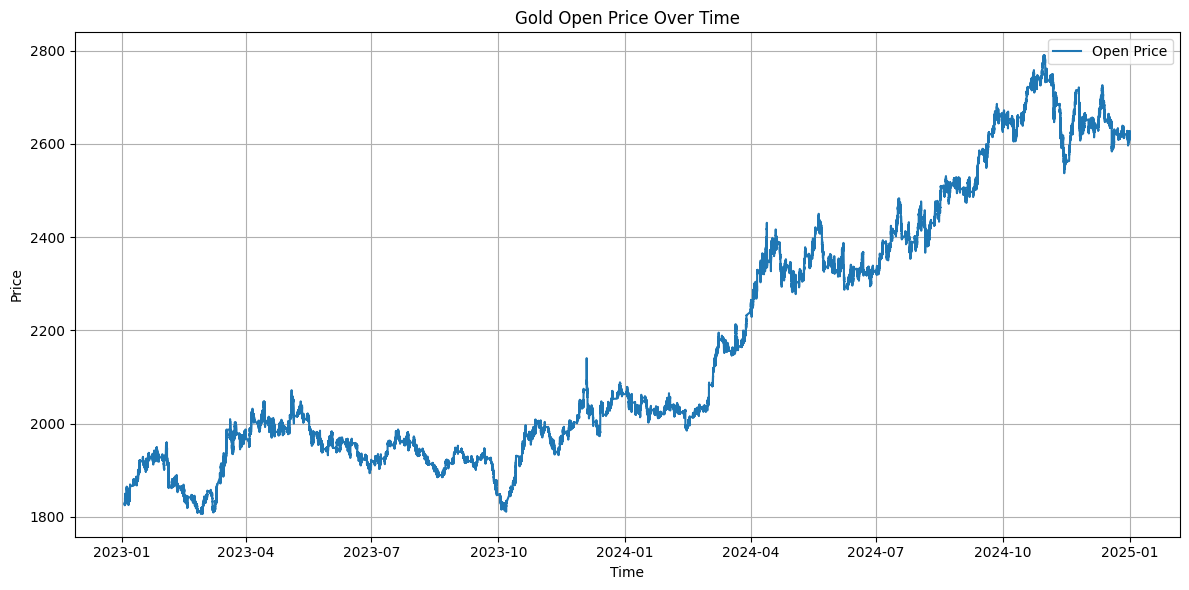
\includegraphics[width=0.8\textwidth]{Figures/Time Series Gold Price.png}
    \caption{Time Series Gold Price}
    \label{fig:time_series_goldprice}
\end{figure}

%--------------------------------------------------------------------------
% 13. August 2025


%\cleardoublepage


\newpage
\section{Portfolio Optimization}
% https://portfoliooptimizationbook.com/

% \cite{palomar:portfolio_optimization}
\newpage
\subsection{Prices and Returns}

The price of an asset $p_t$ is the most obvious quantity, where $t$ is the discrete time index, it can also be continuous.

When it comes to modeling, using the logarithm of the prices enhances the mathematical convenience and also represents a wider dynamic range naturally.

% The simplest model for the log-prices is the random walk


\subsection{Financial Data: I.I.D. Modeling}
EMH: price of security = intrinsic value
any further information about future prospects incorporated in the current price (forecast = current price) 
-> modeling the prices as a random walk $\iff$ returns as a sequence of iid random variables

multiple assets: random variables = return of all assets (multivariate random variable)

under iid: no temporal structure incorporated returns are assumed to be independent distribution of random returns assumed fixed
\subsection{I.I.D. Model}
ignores temporal structures/ dependency in the data
\[x_t = \mu + \epsilon_t\]
\subsection{Sample Estimators}
sample mean
sample covariance matrix
estimators are unbiased and consistent
\subsection{Location Estimators}
\begin{enumerate}
    \item $\textbf{Least square estimator}$
    \item $\textbf{Median estimator}$
    \item $\textbf{Spatial median estimator or geometric median}$
\end{enumerate}

Numerical experiments

For $\textbf{Gaussian data}$, the sample mean is the best estimator (as further analyzed in Section 3.4), the spatial median is almost identical, and the elementwise median is the worst. 
For $\textbf{heavy-tailed data}$, the sample mean is as bad as the median and the spatial median remains the best. 

Overall, the spatial median seems to be the best option as it is robust to outliers and does not underperform under Gaussian data.

\subsection{Gaussian ML estimators}
Maximum likelihood estimation: important technique in estimation theory
likelihood function

pdf to the iid model, assuming that the residual follows a multivariate normal or Gaussian distribution, is 
\[f(x) = \frac{1}{\sqrt{(2\pi)^N|\Sigma|}}exp(-\frac{1}{2}(x-\mu)^\intercal\Sigma^{-1}(x-\mu))\]
%\cleardoublepage


\newpage
\section*{Codes and Explanation}
% Linear Growth Model/ Local Linear Trend State Space Model-------------------
% \cite{triantafyllopoulos:bayesian_state_space}
\subsection*{Local Linear Trend Model}

State Space: 

\textbf{State vector:}
\[x_t= \begin{bmatrix} 
                \mu_t \\ 
                \nu_t 
            \end{bmatrix}\]

where $\mu_t$ is the local level and $\nu_t$ is the local slope.

\textbf{State transition equation:}
$$x_{t+1} = Fx_t + q_t$$ 

with transition matrix
$F=\begin{bmatrix} 
        1 & 1 \\ 
        0 & 1
    \end{bmatrix},$
$q_t = \begin{bmatrix}
    \eta_t \\ \zeta_t
\end{bmatrix}$
and process noise covariance
$Q=\begin{bmatrix} 
        \sigma^2_\eta & 0 \\ 
        0 & \sigma^2_\zeta 
    \end{bmatrix}.$
    
\textbf{Observation equation:}
$$y_t = Hx_t+\epsilon_t, \quad \epsilon_t \sim \mathcal{N}(0, \sigma^2_\epsilon)$$ 

with observation matrix $H=\begin{bmatrix} 1 & 0 \end{bmatrix}.$

\begin{itemize}
    \item $\eta_t$ level noise, 
    \item $\zeta_t$ slope noise and
    \item $\epsilon_t$ observation noise. 

    \item $\nu_t$ follows a linear function and a random error $\zeta_t$
\end{itemize}

\textbf{Component form:}
% component form shows the individual dynamics of \mu_t and \beta_t whereas matrix form is compact and convenient for algorithms (Kalman filter, smoothing)

$$\mu_{t+1} = \mu_t + \nu_t + \eta_t, \quad \eta_t \sim \mathcal{N}(0, \sigma^2_\eta)$$ 
% level: previous level + slope + random noise \eta_t

$$\nu_{t+1} = \nu_t + \zeta_t, \quad \zeta_t \sim \mathcal{N}(0, \sigma^2_\zeta)$$ 
% slope: random walk + noise \zeta_t

$$y_t= \mu_t+\epsilon_t, \quad \epsilon_t \sim \mathcal{N}(0, \sigma^2_\epsilon)$$ 
% observation equation
%\cleardoublepage


% References 
% \printbibliography

\end{document}

